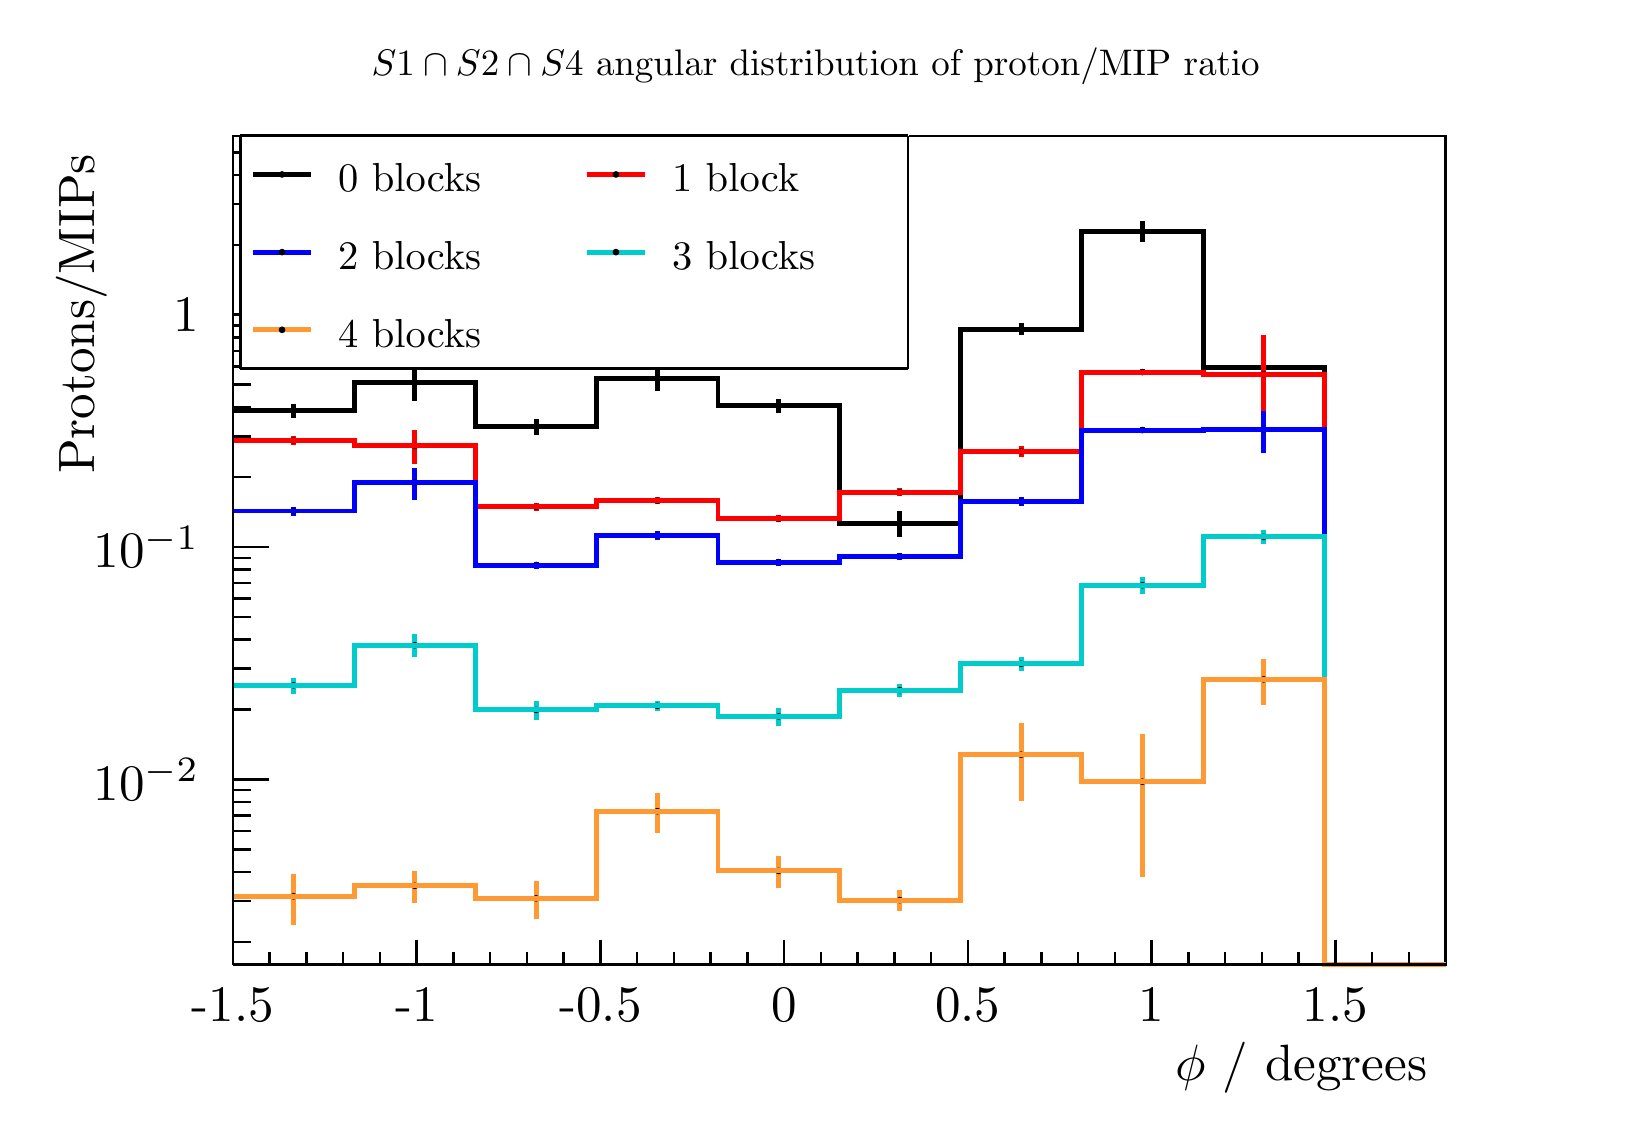
\begin{tikzpicture}
\pgfdeclareplotmark{cross} {
\pgfpathmoveto{\pgfpoint{-0.3\pgfplotmarksize}{\pgfplotmarksize}}
\pgfpathlineto{\pgfpoint{+0.3\pgfplotmarksize}{\pgfplotmarksize}}
\pgfpathlineto{\pgfpoint{+0.3\pgfplotmarksize}{0.3\pgfplotmarksize}}
\pgfpathlineto{\pgfpoint{+1\pgfplotmarksize}{0.3\pgfplotmarksize}}
\pgfpathlineto{\pgfpoint{+1\pgfplotmarksize}{-0.3\pgfplotmarksize}}
\pgfpathlineto{\pgfpoint{+0.3\pgfplotmarksize}{-0.3\pgfplotmarksize}}
\pgfpathlineto{\pgfpoint{+0.3\pgfplotmarksize}{-1.\pgfplotmarksize}}
\pgfpathlineto{\pgfpoint{-0.3\pgfplotmarksize}{-1.\pgfplotmarksize}}
\pgfpathlineto{\pgfpoint{-0.3\pgfplotmarksize}{-0.3\pgfplotmarksize}}
\pgfpathlineto{\pgfpoint{-1.\pgfplotmarksize}{-0.3\pgfplotmarksize}}
\pgfpathlineto{\pgfpoint{-1.\pgfplotmarksize}{0.3\pgfplotmarksize}}
\pgfpathlineto{\pgfpoint{-0.3\pgfplotmarksize}{0.3\pgfplotmarksize}}
\pgfpathclose
\pgfusepathqstroke
}
\pgfdeclareplotmark{cross*} {
\pgfpathmoveto{\pgfpoint{-0.3\pgfplotmarksize}{\pgfplotmarksize}}
\pgfpathlineto{\pgfpoint{+0.3\pgfplotmarksize}{\pgfplotmarksize}}
\pgfpathlineto{\pgfpoint{+0.3\pgfplotmarksize}{0.3\pgfplotmarksize}}
\pgfpathlineto{\pgfpoint{+1\pgfplotmarksize}{0.3\pgfplotmarksize}}
\pgfpathlineto{\pgfpoint{+1\pgfplotmarksize}{-0.3\pgfplotmarksize}}
\pgfpathlineto{\pgfpoint{+0.3\pgfplotmarksize}{-0.3\pgfplotmarksize}}
\pgfpathlineto{\pgfpoint{+0.3\pgfplotmarksize}{-1.\pgfplotmarksize}}
\pgfpathlineto{\pgfpoint{-0.3\pgfplotmarksize}{-1.\pgfplotmarksize}}
\pgfpathlineto{\pgfpoint{-0.3\pgfplotmarksize}{-0.3\pgfplotmarksize}}
\pgfpathlineto{\pgfpoint{-1.\pgfplotmarksize}{-0.3\pgfplotmarksize}}
\pgfpathlineto{\pgfpoint{-1.\pgfplotmarksize}{0.3\pgfplotmarksize}}
\pgfpathlineto{\pgfpoint{-0.3\pgfplotmarksize}{0.3\pgfplotmarksize}}
\pgfpathclose
\pgfusepathqfillstroke
}
\pgfdeclareplotmark{newstar} {
\pgfpathmoveto{\pgfqpoint{0pt}{\pgfplotmarksize}}
\pgfpathlineto{\pgfqpointpolar{44}{0.5\pgfplotmarksize}}
\pgfpathlineto{\pgfqpointpolar{18}{\pgfplotmarksize}}
\pgfpathlineto{\pgfqpointpolar{-20}{0.5\pgfplotmarksize}}
\pgfpathlineto{\pgfqpointpolar{-54}{\pgfplotmarksize}}
\pgfpathlineto{\pgfqpointpolar{-90}{0.5\pgfplotmarksize}}
\pgfpathlineto{\pgfqpointpolar{234}{\pgfplotmarksize}}
\pgfpathlineto{\pgfqpointpolar{198}{0.5\pgfplotmarksize}}
\pgfpathlineto{\pgfqpointpolar{162}{\pgfplotmarksize}}
\pgfpathlineto{\pgfqpointpolar{134}{0.5\pgfplotmarksize}}
\pgfpathclose
\pgfusepathqstroke
}
\pgfdeclareplotmark{newstar*} {
\pgfpathmoveto{\pgfqpoint{0pt}{\pgfplotmarksize}}
\pgfpathlineto{\pgfqpointpolar{44}{0.5\pgfplotmarksize}}
\pgfpathlineto{\pgfqpointpolar{18}{\pgfplotmarksize}}
\pgfpathlineto{\pgfqpointpolar{-20}{0.5\pgfplotmarksize}}
\pgfpathlineto{\pgfqpointpolar{-54}{\pgfplotmarksize}}
\pgfpathlineto{\pgfqpointpolar{-90}{0.5\pgfplotmarksize}}
\pgfpathlineto{\pgfqpointpolar{234}{\pgfplotmarksize}}
\pgfpathlineto{\pgfqpointpolar{198}{0.5\pgfplotmarksize}}
\pgfpathlineto{\pgfqpointpolar{162}{\pgfplotmarksize}}
\pgfpathlineto{\pgfqpointpolar{134}{0.5\pgfplotmarksize}}
\pgfpathclose
\pgfusepathqfillstroke
}
\definecolor{c}{rgb}{1,1,1};
\draw [color=c, fill=c] (0,0) rectangle (20,13.6676);
\draw [color=c, fill=c] (2.6,1.77679) rectangle (18,12.3009);
\definecolor{c}{rgb}{0,0,0};
\draw [c,line width=0.9] (2.6,1.77679) -- (2.6,12.3009) -- (18,12.3009) -- (18,1.77679) -- (2.6,1.77679);
\definecolor{c}{rgb}{1,1,1};
\draw [color=c, fill=c] (2.6,1.77679) rectangle (18,12.3009);
\definecolor{c}{rgb}{0,0,0};
\draw [c,line width=0.9] (2.6,1.77679) -- (2.6,12.3009) -- (18,12.3009) -- (18,1.77679) -- (2.6,1.77679);
\definecolor{c}{rgb}{0,0,0.6};
\draw [c,line width=0.9] (2.6,1.77679) -- (4.14,1.77679) -- (4.14,1.77679) -- (5.68,1.77679) -- (5.68,1.77679) -- (7.22,1.77679) -- (7.22,1.77679) -- (8.76,1.77679) -- (8.76,1.77679) -- (10.3,1.77679) -- (10.3,1.77679) -- (11.84,1.77679) --
 (11.84,1.77679) -- (13.38,1.77679) -- (13.38,1.77679) -- (14.92,1.77679) -- (14.92,1.77679) -- (16.46,1.77679) -- (16.46,1.77679) -- (18,1.77679);
\definecolor{c}{rgb}{0,0,0};
\draw [c,line width=0.9] (2.6,1.77679) -- (18,1.77679);
\draw [c,line width=0.9] (2.6,2.09251) -- (2.6,1.77679);
\draw [c,line width=0.9] (3.06667,1.93465) -- (3.06667,1.77679);
\draw [c,line width=0.9] (3.53333,1.93465) -- (3.53333,1.77679);
\draw [c,line width=0.9] (4,1.93465) -- (4,1.77679);
\draw [c,line width=0.9] (4.46667,1.93465) -- (4.46667,1.77679);
\draw [c,line width=0.9] (4.93333,2.09251) -- (4.93333,1.77679);
\draw [c,line width=0.9] (5.4,1.93465) -- (5.4,1.77679);
\draw [c,line width=0.9] (5.86667,1.93465) -- (5.86667,1.77679);
\draw [c,line width=0.9] (6.33333,1.93465) -- (6.33333,1.77679);
\draw [c,line width=0.9] (6.8,1.93465) -- (6.8,1.77679);
\draw [c,line width=0.9] (7.26667,2.09251) -- (7.26667,1.77679);
\draw [c,line width=0.9] (7.73333,1.93465) -- (7.73333,1.77679);
\draw [c,line width=0.9] (8.2,1.93465) -- (8.2,1.77679);
\draw [c,line width=0.9] (8.66667,1.93465) -- (8.66667,1.77679);
\draw [c,line width=0.9] (9.13333,1.93465) -- (9.13333,1.77679);
\draw [c,line width=0.9] (9.6,2.09251) -- (9.6,1.77679);
\draw [c,line width=0.9] (10.0667,1.93465) -- (10.0667,1.77679);
\draw [c,line width=0.9] (10.5333,1.93465) -- (10.5333,1.77679);
\draw [c,line width=0.9] (11,1.93465) -- (11,1.77679);
\draw [c,line width=0.9] (11.4667,1.93465) -- (11.4667,1.77679);
\draw [c,line width=0.9] (11.9333,2.09251) -- (11.9333,1.77679);
\draw [c,line width=0.9] (12.4,1.93465) -- (12.4,1.77679);
\draw [c,line width=0.9] (12.8667,1.93465) -- (12.8667,1.77679);
\draw [c,line width=0.9] (13.3333,1.93465) -- (13.3333,1.77679);
\draw [c,line width=0.9] (13.8,1.93465) -- (13.8,1.77679);
\draw [c,line width=0.9] (14.2667,2.09251) -- (14.2667,1.77679);
\draw [c,line width=0.9] (14.7333,1.93465) -- (14.7333,1.77679);
\draw [c,line width=0.9] (15.2,1.93465) -- (15.2,1.77679);
\draw [c,line width=0.9] (15.6667,1.93465) -- (15.6667,1.77679);
\draw [c,line width=0.9] (16.1333,1.93465) -- (16.1333,1.77679);
\draw [c,line width=0.9] (16.6,2.09251) -- (16.6,1.77679);
\draw [c,line width=0.9] (16.6,2.09251) -- (16.6,1.77679);
\draw [c,line width=0.9] (17.0667,1.93465) -- (17.0667,1.77679);
\draw [c,line width=0.9] (17.5333,1.93465) -- (17.5333,1.77679);
\draw [anchor=base] (2.6,1.05241) node[scale=1.84551, color=c, rotate=0]{-1.5};
\draw [anchor=base] (4.93333,1.05241) node[scale=1.84551, color=c, rotate=0]{-1};
\draw [anchor=base] (7.26667,1.05241) node[scale=1.84551, color=c, rotate=0]{-0.5};
\draw [anchor=base] (9.6,1.05241) node[scale=1.84551, color=c, rotate=0]{0};
\draw [anchor=base] (11.9333,1.05241) node[scale=1.84551, color=c, rotate=0]{0.5};
\draw [anchor=base] (14.2667,1.05241) node[scale=1.84551, color=c, rotate=0]{1};
\draw [anchor=base] (16.6,1.05241) node[scale=1.84551, color=c, rotate=0]{1.5};
\draw [anchor= east] (18,0.464699) node[scale=1.84551, color=c, rotate=0]{$\phi$ / degrees};
\draw [c,line width=0.9] (2.6,1.77679) -- (2.6,12.3009);
\draw [c,line width=0.9] (2.831,2.06283) -- (2.6,2.06283);
\draw [c,line width=0.9] (2.831,2.58255) -- (2.6,2.58255);
\draw [c,line width=0.9] (2.831,2.9513) -- (2.6,2.9513);
\draw [c,line width=0.9] (2.831,3.23732) -- (2.6,3.23732);
\draw [c,line width=0.9] (2.831,3.47102) -- (2.6,3.47102);
\draw [c,line width=0.9] (2.831,3.66861) -- (2.6,3.66861);
\draw [c,line width=0.9] (2.831,3.83977) -- (2.6,3.83977);
\draw [c,line width=0.9] (2.831,3.99075) -- (2.6,3.99075);
\draw [c,line width=0.9] (3.062,4.1258) -- (2.6,4.1258);
\draw [anchor= east] (2.404,4.1258) node[scale=1.84551, color=c, rotate=0]{$10^{-2}$};
\draw [c,line width=0.9] (2.831,5.01427) -- (2.6,5.01427);
\draw [c,line width=0.9] (2.831,5.53399) -- (2.6,5.53399);
\draw [c,line width=0.9] (2.831,5.90274) -- (2.6,5.90274);
\draw [c,line width=0.9] (2.831,6.18877) -- (2.6,6.18877);
\draw [c,line width=0.9] (2.831,6.42247) -- (2.6,6.42247);
\draw [c,line width=0.9] (2.831,6.62006) -- (2.6,6.62006);
\draw [c,line width=0.9] (2.831,6.79122) -- (2.6,6.79122);
\draw [c,line width=0.9] (2.831,6.94219) -- (2.6,6.94219);
\draw [c,line width=0.9] (3.062,7.07724) -- (2.6,7.07724);
\draw [anchor= east] (2.404,7.07724) node[scale=1.84551, color=c, rotate=0]{$10^{-1}$};
\draw [c,line width=0.9] (2.831,7.96572) -- (2.6,7.96572);
\draw [c,line width=0.9] (2.831,8.48544) -- (2.6,8.48544);
\draw [c,line width=0.9] (2.831,8.85419) -- (2.6,8.85419);
\draw [c,line width=0.9] (2.831,9.14021) -- (2.6,9.14021);
\draw [c,line width=0.9] (2.831,9.37391) -- (2.6,9.37391);
\draw [c,line width=0.9] (2.831,9.5715) -- (2.6,9.5715);
\draw [c,line width=0.9] (2.831,9.74266) -- (2.6,9.74266);
\draw [c,line width=0.9] (2.831,9.89364) -- (2.6,9.89364);
\draw [c,line width=0.9] (3.062,10.0287) -- (2.6,10.0287);
\draw [anchor= east] (2.404,10.0287) node[scale=1.84551, color=c, rotate=0]{1};
\draw [c,line width=0.9] (2.831,10.9172) -- (2.6,10.9172);
\draw [c,line width=0.9] (2.831,11.4369) -- (2.6,11.4369);
\draw [c,line width=0.9] (2.831,11.8056) -- (2.6,11.8056);
\draw [c,line width=0.9] (2.831,12.0917) -- (2.6,12.0917);
\draw [anchor= east] (0.68,12.3009) node[scale=1.84551, color=c, rotate=90]{ Protons/MIPs};
\draw [c,line width=1.8] (3.37,8.71572) -- (3.37,8.80933);
\draw [c,line width=1.8] (3.37,8.80933) -- (3.37,8.89657);
\foreach \P in {(3.37,8.80933)}{\draw[mark options={color=c,fill=c},mark size=2.402402pt,mark=*,mark size=1pt] plot coordinates {\P};}
\draw [c,line width=1.8] (4.91,8.93264) -- (4.91,9.16546);
\draw [c,line width=1.8] (4.91,9.16546) -- (4.91,9.36243);
\foreach \P in {(4.91,9.16546)}{\draw[mark options={color=c,fill=c},mark size=2.402402pt,mark=*,mark size=1pt] plot coordinates {\P};}
\draw [c,line width=1.8] (6.45,8.50034) -- (6.45,8.60794);
\draw [c,line width=1.8] (6.45,8.60794) -- (6.45,8.7072);
\foreach \P in {(6.45,8.60794)}{\draw[mark options={color=c,fill=c},mark size=2.402402pt,mark=*,mark size=1pt] plot coordinates {\P};}
\draw [c,line width=1.8] (7.99,9.0555) -- (7.99,9.21617);
\draw [c,line width=1.8] (7.99,9.21617) -- (7.99,9.35892);
\foreach \P in {(7.99,9.21617)}{\draw[mark options={color=c,fill=c},mark size=2.402402pt,mark=*,mark size=1pt] plot coordinates {\P};}
\draw [c,line width=1.8] (9.53,8.77724) -- (9.53,8.87212);
\draw [c,line width=1.8] (9.53,8.87212) -- (9.53,8.96046);
\foreach \P in {(9.53,8.87212)}{\draw[mark options={color=c,fill=c},mark size=2.402402pt,mark=*,mark size=1pt] plot coordinates {\P};}
\draw [c,line width=1.8] (11.07,7.20089) -- (11.07,7.37832);
\draw [c,line width=1.8] (11.07,7.37832) -- (11.07,7.53414);
\foreach \P in {(11.07,7.37832)}{\draw[mark options={color=c,fill=c},mark size=2.402402pt,mark=*,mark size=1pt] plot coordinates {\P};}
\draw [c,line width=1.8] (12.61,9.76905) -- (12.61,9.84608);
\draw [c,line width=1.8] (12.61,9.84608) -- (12.61,9.91874);
\foreach \P in {(12.61,9.84608)}{\draw[mark options={color=c,fill=c},mark size=2.402402pt,mark=*,mark size=1pt] plot coordinates {\P};}
\draw [c,line width=1.8] (14.15,10.9512) -- (14.15,11.0904);
\draw [c,line width=1.8] (14.15,11.0904) -- (14.15,11.2159);
\foreach \P in {(14.15,11.0904)}{\draw[mark options={color=c,fill=c},mark size=2.402402pt,mark=*,mark size=1pt] plot coordinates {\P};}
\draw [c,line width=1.8] (15.69,8.97735) -- (15.69,9.35255);
\draw [c,line width=1.8] (15.69,9.35255) -- (15.69,9.64243);
\foreach \P in {(15.69,9.35255)}{\draw[mark options={color=c,fill=c},mark size=2.402402pt,mark=*,mark size=1pt] plot coordinates {\P};}
\draw [c,line width=1.8] (2.6,8.80933) -- (4.14,8.80933) -- (4.14,9.16546) -- (5.68,9.16546) -- (5.68,8.60794) -- (7.22,8.60794) -- (7.22,9.21617) -- (8.76,9.21617) -- (8.76,8.87212) -- (10.3,8.87212) -- (10.3,7.37832) -- (11.84,7.37832) --
 (11.84,9.84608) -- (13.38,9.84608) -- (13.38,11.0904) -- (14.92,11.0904) -- (14.92,9.35255) -- (16.46,9.35255) -- (16.46,1.77679) -- (18,1.77679);
\definecolor{c}{rgb}{1,0,0};
\draw [c,line width=1.8] (3.37,8.37421) -- (3.37,8.43149);
\draw [c,line width=1.8] (3.37,8.43149) -- (3.37,8.48632);
\definecolor{c}{rgb}{0,0,0};
\foreach \P in {(3.37,8.43149)}{\draw[mark options={color=c,fill=c},mark size=2.402402pt,mark=*,mark size=1pt] plot coordinates {\P};}
\definecolor{c}{rgb}{1,0,0};
\draw [c,line width=1.8] (4.91,8.12866) -- (4.91,8.3624);
\draw [c,line width=1.8] (4.91,8.3624) -- (4.91,8.56002);
\definecolor{c}{rgb}{0,0,0};
\foreach \P in {(4.91,8.3624)}{\draw[mark options={color=c,fill=c},mark size=2.402402pt,mark=*,mark size=1pt] plot coordinates {\P};}
\definecolor{c}{rgb}{1,0,0};
\draw [c,line width=1.8] (6.45,7.53767) -- (6.45,7.58904);
\draw [c,line width=1.8] (6.45,7.58904) -- (6.45,7.63842);
\definecolor{c}{rgb}{0,0,0};
\foreach \P in {(6.45,7.58904)}{\draw[mark options={color=c,fill=c},mark size=2.402402pt,mark=*,mark size=1pt] plot coordinates {\P};}
\definecolor{c}{rgb}{1,0,0};
\draw [c,line width=1.8] (7.99,7.62578) -- (7.99,7.6677);
\draw [c,line width=1.8] (7.99,7.6677) -- (7.99,7.7083);
\definecolor{c}{rgb}{0,0,0};
\foreach \P in {(7.99,7.6677)}{\draw[mark options={color=c,fill=c},mark size=2.402402pt,mark=*,mark size=1pt] plot coordinates {\P};}
\definecolor{c}{rgb}{1,0,0};
\draw [c,line width=1.8] (9.53,7.39423) -- (9.53,7.43841);
\draw [c,line width=1.8] (9.53,7.43841) -- (9.53,7.48111);
\definecolor{c}{rgb}{0,0,0};
\foreach \P in {(9.53,7.43841)}{\draw[mark options={color=c,fill=c},mark size=2.402402pt,mark=*,mark size=1pt] plot coordinates {\P};}
\definecolor{c}{rgb}{1,0,0};
\draw [c,line width=1.8] (11.07,7.72514) -- (11.07,7.77571);
\draw [c,line width=1.8] (11.07,7.77571) -- (11.07,7.82436);
\definecolor{c}{rgb}{0,0,0};
\foreach \P in {(11.07,7.77571)}{\draw[mark options={color=c,fill=c},mark size=2.402402pt,mark=*,mark size=1pt] plot coordinates {\P};}
\definecolor{c}{rgb}{1,0,0};
\draw [c,line width=1.8] (12.61,8.21721) -- (12.61,8.29447);
\draw [c,line width=1.8] (12.61,8.29447) -- (12.61,8.36734);
\definecolor{c}{rgb}{0,0,0};
\foreach \P in {(12.61,8.29447)}{\draw[mark options={color=c,fill=c},mark size=2.402402pt,mark=*,mark size=1pt] plot coordinates {\P};}
\definecolor{c}{rgb}{1,0,0};
\draw [c,line width=1.8] (14.15,9.265) -- (14.15,9.30053);
\draw [c,line width=1.8] (14.15,9.30053) -- (14.15,9.3351);
\definecolor{c}{rgb}{0,0,0};
\foreach \P in {(14.15,9.30053)}{\draw[mark options={color=c,fill=c},mark size=2.402402pt,mark=*,mark size=1pt] plot coordinates {\P};}
\definecolor{c}{rgb}{1,0,0};
\draw [c,line width=1.8] (15.69,8.44913) -- (15.69,9.27216);
\draw [c,line width=1.8] (15.69,9.27216) -- (15.69,9.76931);
\definecolor{c}{rgb}{0,0,0};
\foreach \P in {(15.69,9.27216)}{\draw[mark options={color=c,fill=c},mark size=2.402402pt,mark=*,mark size=1pt] plot coordinates {\P};}
\definecolor{c}{rgb}{1,0,0};
\draw [c,line width=1.8] (2.6,8.43149) -- (4.14,8.43149) -- (4.14,8.3624) -- (5.68,8.3624) -- (5.68,7.58904) -- (7.22,7.58904) -- (7.22,7.6677) -- (8.76,7.6677) -- (8.76,7.43841) -- (10.3,7.43841) -- (10.3,7.77571) -- (11.84,7.77571) --
 (11.84,8.29447) -- (13.38,8.29447) -- (13.38,9.30053) -- (14.92,9.30053) -- (14.92,9.27216) -- (16.46,9.27216) -- (16.46,1.77679) -- (18,1.77679);
\definecolor{c}{rgb}{0,0,1};
\draw [c,line width=1.8] (3.37,7.47813) -- (3.37,7.53627);
\draw [c,line width=1.8] (3.37,7.53627) -- (3.37,7.59189);
\definecolor{c}{rgb}{0,0,0};
\foreach \P in {(3.37,7.53627)}{\draw[mark options={color=c,fill=c},mark size=2.402402pt,mark=*,mark size=1pt] plot coordinates {\P};}
\definecolor{c}{rgb}{0,0,1};
\draw [c,line width=1.8] (4.91,7.6823) -- (4.91,7.89709);
\draw [c,line width=1.8] (4.91,7.89709) -- (4.91,8.08099);
\definecolor{c}{rgb}{0,0,0};
\foreach \P in {(4.91,7.89709)}{\draw[mark options={color=c,fill=c},mark size=2.402402pt,mark=*,mark size=1pt] plot coordinates {\P};}
\definecolor{c}{rgb}{0,0,1};
\draw [c,line width=1.8] (6.45,6.80451) -- (6.45,6.84936);
\draw [c,line width=1.8] (6.45,6.84936) -- (6.45,6.89269);
\definecolor{c}{rgb}{0,0,0};
\foreach \P in {(6.45,6.84936)}{\draw[mark options={color=c,fill=c},mark size=2.402402pt,mark=*,mark size=1pt] plot coordinates {\P};}
\definecolor{c}{rgb}{0,0,1};
\draw [c,line width=1.8] (7.99,7.16257) -- (7.99,7.2232);
\draw [c,line width=1.8] (7.99,7.2232) -- (7.99,7.28108);
\definecolor{c}{rgb}{0,0,0};
\foreach \P in {(7.99,7.2232)}{\draw[mark options={color=c,fill=c},mark size=2.402402pt,mark=*,mark size=1pt] plot coordinates {\P};}
\definecolor{c}{rgb}{0,0,1};
\draw [c,line width=1.8] (9.53,6.84149) -- (9.53,6.88645);
\draw [c,line width=1.8] (9.53,6.88645) -- (9.53,6.92988);
\definecolor{c}{rgb}{0,0,0};
\foreach \P in {(9.53,6.88645)}{\draw[mark options={color=c,fill=c},mark size=2.402402pt,mark=*,mark size=1pt] plot coordinates {\P};}
\definecolor{c}{rgb}{0,0,1};
\draw [c,line width=1.8] (11.07,6.91345) -- (11.07,6.96148);
\draw [c,line width=1.8] (11.07,6.96148) -- (11.07,7.00777);
\definecolor{c}{rgb}{0,0,0};
\foreach \P in {(11.07,6.96148)}{\draw[mark options={color=c,fill=c},mark size=2.402402pt,mark=*,mark size=1pt] plot coordinates {\P};}
\definecolor{c}{rgb}{0,0,1};
\draw [c,line width=1.8] (12.61,7.60148) -- (12.61,7.65841);
\draw [c,line width=1.8] (12.61,7.65841) -- (12.61,7.71291);
\definecolor{c}{rgb}{0,0,0};
\foreach \P in {(12.61,7.65841)}{\draw[mark options={color=c,fill=c},mark size=2.402402pt,mark=*,mark size=1pt] plot coordinates {\P};}
\definecolor{c}{rgb}{0,0,1};
\draw [c,line width=1.8] (14.15,8.52768) -- (14.15,8.56428);
\draw [c,line width=1.8] (14.15,8.56428) -- (14.15,8.59986);
\definecolor{c}{rgb}{0,0,0};
\foreach \P in {(14.15,8.56428)}{\draw[mark options={color=c,fill=c},mark size=2.402402pt,mark=*,mark size=1pt] plot coordinates {\P};}
\definecolor{c}{rgb}{0,0,1};
\draw [c,line width=1.8] (15.69,8.26831) -- (15.69,8.56877);
\draw [c,line width=1.8] (15.69,8.56877) -- (15.69,8.812);
\definecolor{c}{rgb}{0,0,0};
\foreach \P in {(15.69,8.56877)}{\draw[mark options={color=c,fill=c},mark size=2.402402pt,mark=*,mark size=1pt] plot coordinates {\P};}
\definecolor{c}{rgb}{0,0,1};
\draw [c,line width=1.8] (2.6,7.53627) -- (4.14,7.53627) -- (4.14,7.89709) -- (5.68,7.89709) -- (5.68,6.84936) -- (7.22,6.84936) -- (7.22,7.2232) -- (8.76,7.2232) -- (8.76,6.88645) -- (10.3,6.88645) -- (10.3,6.96148) -- (11.84,6.96148) --
 (11.84,7.65841) -- (13.38,7.65841) -- (13.38,8.56428) -- (14.92,8.56428) -- (14.92,8.56877) -- (16.46,8.56877) -- (16.46,1.77679) -- (18,1.77679);
\definecolor{c}{rgb}{0,0.8,0.8};
\draw [c,line width=1.8] (3.37,5.21736) -- (3.37,5.32217);
\draw [c,line width=1.8] (3.37,5.32217) -- (3.37,5.41905);
\definecolor{c}{rgb}{0,0,0};
\foreach \P in {(3.37,5.32217)}{\draw[mark options={color=c,fill=c},mark size=2.402402pt,mark=*,mark size=1pt] plot coordinates {\P};}
\definecolor{c}{rgb}{0,0.8,0.8};
\draw [c,line width=1.8] (4.91,5.67773) -- (4.91,5.83146);
\draw [c,line width=1.8] (4.91,5.83146) -- (4.91,5.96872);
\definecolor{c}{rgb}{0,0,0};
\foreach \P in {(4.91,5.83146)}{\draw[mark options={color=c,fill=c},mark size=2.402402pt,mark=*,mark size=1pt] plot coordinates {\P};}
\definecolor{c}{rgb}{0,0.8,0.8};
\draw [c,line width=1.8] (6.45,4.88143) -- (6.45,5.01024);
\draw [c,line width=1.8] (6.45,5.01024) -- (6.45,5.12728);
\definecolor{c}{rgb}{0,0,0};
\foreach \P in {(6.45,5.01024)}{\draw[mark options={color=c,fill=c},mark size=2.402402pt,mark=*,mark size=1pt] plot coordinates {\P};}
\definecolor{c}{rgb}{0,0.8,0.8};
\draw [c,line width=1.8] (7.99,4.99179) -- (7.99,5.06237);
\draw [c,line width=1.8] (7.99,5.06237) -- (7.99,5.12926);
\definecolor{c}{rgb}{0,0,0};
\foreach \P in {(7.99,5.06237)}{\draw[mark options={color=c,fill=c},mark size=2.402402pt,mark=*,mark size=1pt] plot coordinates {\P};}
\definecolor{c}{rgb}{0,0.8,0.8};
\draw [c,line width=1.8] (9.53,4.80377) -- (9.53,4.92749);
\draw [c,line width=1.8] (9.53,4.92749) -- (9.53,5.04031);
\definecolor{c}{rgb}{0,0,0};
\foreach \P in {(9.53,4.92749)}{\draw[mark options={color=c,fill=c},mark size=2.402402pt,mark=*,mark size=1pt] plot coordinates {\P};}
\definecolor{c}{rgb}{0,0.8,0.8};
\draw [c,line width=1.8] (11.07,5.1801) -- (11.07,5.26136);
\draw [c,line width=1.8] (11.07,5.26136) -- (11.07,5.33777);
\definecolor{c}{rgb}{0,0,0};
\foreach \P in {(11.07,5.26136)}{\draw[mark options={color=c,fill=c},mark size=2.402402pt,mark=*,mark size=1pt] plot coordinates {\P};}
\definecolor{c}{rgb}{0,0.8,0.8};
\draw [c,line width=1.8] (12.61,5.50823) -- (12.61,5.59604);
\draw [c,line width=1.8] (12.61,5.59604) -- (12.61,5.67821);
\definecolor{c}{rgb}{0,0,0};
\foreach \P in {(12.61,5.59604)}{\draw[mark options={color=c,fill=c},mark size=2.402402pt,mark=*,mark size=1pt] plot coordinates {\P};}
\definecolor{c}{rgb}{0,0.8,0.8};
\draw [c,line width=1.8] (14.15,6.47749) -- (14.15,6.59335);
\draw [c,line width=1.8] (14.15,6.59335) -- (14.15,6.6996);
\definecolor{c}{rgb}{0,0,0};
\foreach \P in {(14.15,6.59335)}{\draw[mark options={color=c,fill=c},mark size=2.402402pt,mark=*,mark size=1pt] plot coordinates {\P};}
\definecolor{c}{rgb}{0,0.8,0.8};
\draw [c,line width=1.8] (15.69,7.11306) -- (15.69,7.2079);
\draw [c,line width=1.8] (15.69,7.2079) -- (15.69,7.2962);
\definecolor{c}{rgb}{0,0,0};
\foreach \P in {(15.69,7.2079)}{\draw[mark options={color=c,fill=c},mark size=2.402402pt,mark=*,mark size=1pt] plot coordinates {\P};}
\definecolor{c}{rgb}{0,0.8,0.8};
\draw [c,line width=1.8] (2.6,5.32217) -- (4.14,5.32217) -- (4.14,5.83146) -- (5.68,5.83146) -- (5.68,5.01024) -- (7.22,5.01024) -- (7.22,5.06237) -- (8.76,5.06237) -- (8.76,4.92749) -- (10.3,4.92749) -- (10.3,5.26136) -- (11.84,5.26136) --
 (11.84,5.59604) -- (13.38,5.59604) -- (13.38,6.59335) -- (14.92,6.59335) -- (14.92,7.2079) -- (16.46,7.2079) -- (16.46,1.77679) -- (18,1.77679);
\definecolor{c}{rgb}{1,0.6,0.2};
\draw [c,line width=1.8] (3.37,2.2785) -- (3.37,2.64315);
\draw [c,line width=1.8] (3.37,2.64315) -- (3.37,2.92671);
\definecolor{c}{rgb}{0,0,0};
\foreach \P in {(3.37,2.64315)}{\draw[mark options={color=c,fill=c},mark size=2.402402pt,mark=*,mark size=1pt] plot coordinates {\P};}
\definecolor{c}{rgb}{1,0.6,0.2};
\draw [c,line width=1.8] (4.91,2.55603) -- (4.91,2.77575);
\draw [c,line width=1.8] (4.91,2.77575) -- (4.91,2.96327);
\definecolor{c}{rgb}{0,0,0};
\foreach \P in {(4.91,2.77575)}{\draw[mark options={color=c,fill=c},mark size=2.402402pt,mark=*,mark size=1pt] plot coordinates {\P};}
\definecolor{c}{rgb}{1,0.6,0.2};
\draw [c,line width=1.8] (6.45,2.35011) -- (6.45,2.61696);
\draw [c,line width=1.8] (6.45,2.61696) -- (6.45,2.83772);
\definecolor{c}{rgb}{0,0,0};
\foreach \P in {(6.45,2.61696)}{\draw[mark options={color=c,fill=c},mark size=2.402402pt,mark=*,mark size=1pt] plot coordinates {\P};}
\definecolor{c}{rgb}{1,0.6,0.2};
\draw [c,line width=1.8] (7.99,3.4503) -- (7.99,3.72392);
\draw [c,line width=1.8] (7.99,3.72392) -- (7.99,3.94928);
\definecolor{c}{rgb}{0,0,0};
\foreach \P in {(7.99,3.72392)}{\draw[mark options={color=c,fill=c},mark size=2.402402pt,mark=*,mark size=1pt] plot coordinates {\P};}
\definecolor{c}{rgb}{1,0.6,0.2};
\draw [c,line width=1.8] (9.53,2.75013) -- (9.53,2.96548);
\draw [c,line width=1.8] (9.53,2.96548) -- (9.53,3.1498);
\definecolor{c}{rgb}{0,0,0};
\foreach \P in {(9.53,2.96548)}{\draw[mark options={color=c,fill=c},mark size=2.402402pt,mark=*,mark size=1pt] plot coordinates {\P};}
\definecolor{c}{rgb}{1,0.6,0.2};
\draw [c,line width=1.8] (11.07,2.45532) -- (11.07,2.59494);
\draw [c,line width=1.8] (11.07,2.59494) -- (11.07,2.72083);
\definecolor{c}{rgb}{0,0,0};
\foreach \P in {(11.07,2.59494)}{\draw[mark options={color=c,fill=c},mark size=2.402402pt,mark=*,mark size=1pt] plot coordinates {\P};}
\definecolor{c}{rgb}{1,0.6,0.2};
\draw [c,line width=1.8] (12.61,3.85024) -- (12.61,4.44126);
\draw [c,line width=1.8] (12.61,4.44126) -- (12.61,4.84423);
\definecolor{c}{rgb}{0,0,0};
\foreach \P in {(12.61,4.44126)}{\draw[mark options={color=c,fill=c},mark size=2.402402pt,mark=*,mark size=1pt] plot coordinates {\P};}
\definecolor{c}{rgb}{1,0.6,0.2};
\draw [c,line width=1.8] (14.15,2.88649) -- (14.15,4.09811);
\draw [c,line width=1.8] (14.15,4.09811) -- (14.15,4.70967);
\definecolor{c}{rgb}{0,0,0};
\foreach \P in {(14.15,4.09811)}{\draw[mark options={color=c,fill=c},mark size=2.402402pt,mark=*,mark size=1pt] plot coordinates {\P};}
\definecolor{c}{rgb}{1,0.6,0.2};
\draw [c,line width=1.8] (15.69,5.07692) -- (15.69,5.39867);
\draw [c,line width=1.8] (15.69,5.39867) -- (15.69,5.65564);
\definecolor{c}{rgb}{0,0,0};
\foreach \P in {(15.69,5.39867)}{\draw[mark options={color=c,fill=c},mark size=2.402402pt,mark=*,mark size=1pt] plot coordinates {\P};}
\definecolor{c}{rgb}{1,0.6,0.2};
\draw [c,line width=1.8] (2.6,2.64315) -- (4.14,2.64315) -- (4.14,2.77575) -- (5.68,2.77575) -- (5.68,2.61696) -- (7.22,2.61696) -- (7.22,3.72392) -- (8.76,3.72392) -- (8.76,2.96548) -- (10.3,2.96548) -- (10.3,2.59494) -- (11.84,2.59494) --
 (11.84,4.44126) -- (13.38,4.44126) -- (13.38,4.09811) -- (14.92,4.09811) -- (14.92,5.39867) -- (16.46,5.39867) -- (16.46,1.77679) -- (18,1.77679);
\definecolor{c}{rgb}{0,0,0};
\draw [c,line width=0.9] (2.6,1.77679) -- (18,1.77679);
\draw [c,line width=0.9] (2.6,2.09251) -- (2.6,1.77679);
\draw [c,line width=0.9] (3.06667,1.93465) -- (3.06667,1.77679);
\draw [c,line width=0.9] (3.53333,1.93465) -- (3.53333,1.77679);
\draw [c,line width=0.9] (4,1.93465) -- (4,1.77679);
\draw [c,line width=0.9] (4.46667,1.93465) -- (4.46667,1.77679);
\draw [c,line width=0.9] (4.93333,2.09251) -- (4.93333,1.77679);
\draw [c,line width=0.9] (5.4,1.93465) -- (5.4,1.77679);
\draw [c,line width=0.9] (5.86667,1.93465) -- (5.86667,1.77679);
\draw [c,line width=0.9] (6.33333,1.93465) -- (6.33333,1.77679);
\draw [c,line width=0.9] (6.8,1.93465) -- (6.8,1.77679);
\draw [c,line width=0.9] (7.26667,2.09251) -- (7.26667,1.77679);
\draw [c,line width=0.9] (7.73333,1.93465) -- (7.73333,1.77679);
\draw [c,line width=0.9] (8.2,1.93465) -- (8.2,1.77679);
\draw [c,line width=0.9] (8.66667,1.93465) -- (8.66667,1.77679);
\draw [c,line width=0.9] (9.13333,1.93465) -- (9.13333,1.77679);
\draw [c,line width=0.9] (9.6,2.09251) -- (9.6,1.77679);
\draw [c,line width=0.9] (10.0667,1.93465) -- (10.0667,1.77679);
\draw [c,line width=0.9] (10.5333,1.93465) -- (10.5333,1.77679);
\draw [c,line width=0.9] (11,1.93465) -- (11,1.77679);
\draw [c,line width=0.9] (11.4667,1.93465) -- (11.4667,1.77679);
\draw [c,line width=0.9] (11.9333,2.09251) -- (11.9333,1.77679);
\draw [c,line width=0.9] (12.4,1.93465) -- (12.4,1.77679);
\draw [c,line width=0.9] (12.8667,1.93465) -- (12.8667,1.77679);
\draw [c,line width=0.9] (13.3333,1.93465) -- (13.3333,1.77679);
\draw [c,line width=0.9] (13.8,1.93465) -- (13.8,1.77679);
\draw [c,line width=0.9] (14.2667,2.09251) -- (14.2667,1.77679);
\draw [c,line width=0.9] (14.7333,1.93465) -- (14.7333,1.77679);
\draw [c,line width=0.9] (15.2,1.93465) -- (15.2,1.77679);
\draw [c,line width=0.9] (15.6667,1.93465) -- (15.6667,1.77679);
\draw [c,line width=0.9] (16.1333,1.93465) -- (16.1333,1.77679);
\draw [c,line width=0.9] (16.6,2.09251) -- (16.6,1.77679);
\draw [c,line width=0.9] (16.6,2.09251) -- (16.6,1.77679);
\draw [c,line width=0.9] (17.0667,1.93465) -- (17.0667,1.77679);
\draw [c,line width=0.9] (17.5333,1.93465) -- (17.5333,1.77679);
\draw [c,line width=0.9] (2.6,1.77679) -- (2.6,12.3009);
\draw [c,line width=0.9] (2.831,2.06283) -- (2.6,2.06283);
\draw [c,line width=0.9] (2.831,2.58255) -- (2.6,2.58255);
\draw [c,line width=0.9] (2.831,2.9513) -- (2.6,2.9513);
\draw [c,line width=0.9] (2.831,3.23732) -- (2.6,3.23732);
\draw [c,line width=0.9] (2.831,3.47102) -- (2.6,3.47102);
\draw [c,line width=0.9] (2.831,3.66861) -- (2.6,3.66861);
\draw [c,line width=0.9] (2.831,3.83977) -- (2.6,3.83977);
\draw [c,line width=0.9] (2.831,3.99075) -- (2.6,3.99075);
\draw [c,line width=0.9] (3.062,4.1258) -- (2.6,4.1258);
\draw [c,line width=0.9] (2.831,5.01427) -- (2.6,5.01427);
\draw [c,line width=0.9] (2.831,5.53399) -- (2.6,5.53399);
\draw [c,line width=0.9] (2.831,5.90274) -- (2.6,5.90274);
\draw [c,line width=0.9] (2.831,6.18877) -- (2.6,6.18877);
\draw [c,line width=0.9] (2.831,6.42247) -- (2.6,6.42247);
\draw [c,line width=0.9] (2.831,6.62006) -- (2.6,6.62006);
\draw [c,line width=0.9] (2.831,6.79122) -- (2.6,6.79122);
\draw [c,line width=0.9] (2.831,6.94219) -- (2.6,6.94219);
\draw [c,line width=0.9] (3.062,7.07724) -- (2.6,7.07724);
\draw [c,line width=0.9] (2.831,7.96572) -- (2.6,7.96572);
\draw [c,line width=0.9] (2.831,8.48544) -- (2.6,8.48544);
\draw [c,line width=0.9] (2.831,8.85419) -- (2.6,8.85419);
\draw [c,line width=0.9] (2.831,9.14021) -- (2.6,9.14021);
\draw [c,line width=0.9] (2.831,9.37391) -- (2.6,9.37391);
\draw [c,line width=0.9] (2.831,9.5715) -- (2.6,9.5715);
\draw [c,line width=0.9] (2.831,9.74266) -- (2.6,9.74266);
\draw [c,line width=0.9] (2.831,9.89364) -- (2.6,9.89364);
\draw [c,line width=0.9] (3.062,10.0287) -- (2.6,10.0287);
\draw [c,line width=0.9] (2.831,10.9172) -- (2.6,10.9172);
\draw [c,line width=0.9] (2.831,11.4369) -- (2.6,11.4369);
\draw [c,line width=0.9] (2.831,11.8056) -- (2.6,11.8056);
\draw [c,line width=0.9] (2.831,12.0917) -- (2.6,12.0917);
\draw (10,13.1814) node[scale=1.3364, color=c, rotate=0]{$S1 \cap S2 \cap S4$ angular distribution of proton/MIP ratio};
\definecolor{c}{rgb}{1,1,1};
\draw [color=c, fill=c] (2.69341,9.34389) rectangle (11.1748,12.3038);
\definecolor{c}{rgb}{0,0,0};
\draw [c,line width=0.9] (2.69341,9.34389) -- (11.1748,9.34389);
\draw [c,line width=0.9] (11.1748,9.34389) -- (11.1748,12.3038);
\draw [c,line width=0.9] (11.1748,12.3038) -- (2.69341,12.3038);
\draw [c,line width=0.9] (2.69341,12.3038) -- (2.69341,9.34389);
\draw [anchor=base west] (3.75358,11.5885) node[scale=1.46368, color=c, rotate=0]{0 blocks};
\definecolor{c}{rgb}{1,1,1};
\draw [c, fill=c] (2.85244,11.4651) -- (3.59456,11.4651) -- (3.59456,12.1558) -- (2.85244,12.1558);
\definecolor{c}{rgb}{0,0,0};
\draw [c,line width=1.8] (2.85244,11.8105) -- (3.59456,11.8105);
\foreach \P in {(3.2235,11.8105)}{\draw[mark options={color=c,fill=c},mark size=2.402402pt,mark=*,mark size=1pt] plot coordinates {\P};}
\draw [anchor=base west] (7.99427,11.5885) node[scale=1.46368, color=c, rotate=0]{1 block};
\definecolor{c}{rgb}{1,1,1};
\draw [c, fill=c] (7.09312,11.4651) -- (7.83524,11.4651) -- (7.83524,12.1558) -- (7.09312,12.1558);
\definecolor{c}{rgb}{1,0,0};
\draw [c,line width=1.8] (7.09312,11.8105) -- (7.83524,11.8105);
\definecolor{c}{rgb}{0,0,0};
\foreach \P in {(7.46418,11.8105)}{\draw[mark options={color=c,fill=c},mark size=2.402402pt,mark=*,mark size=1pt] plot coordinates {\P};}
\draw [anchor=base west] (3.75358,10.6018) node[scale=1.46368, color=c, rotate=0]{2 blocks};
\definecolor{c}{rgb}{1,1,1};
\draw [c, fill=c] (2.85244,10.4785) -- (3.59456,10.4785) -- (3.59456,11.1691) -- (2.85244,11.1691);
\definecolor{c}{rgb}{0,0,1};
\draw [c,line width=1.8] (2.85244,10.8238) -- (3.59456,10.8238);
\definecolor{c}{rgb}{0,0,0};
\foreach \P in {(3.2235,10.8238)}{\draw[mark options={color=c,fill=c},mark size=2.402402pt,mark=*,mark size=1pt] plot coordinates {\P};}
\draw [anchor=base west] (7.99427,10.6018) node[scale=1.46368, color=c, rotate=0]{3 blocks};
\definecolor{c}{rgb}{1,1,1};
\draw [c, fill=c] (7.09312,10.4785) -- (7.83524,10.4785) -- (7.83524,11.1691) -- (7.09312,11.1691);
\definecolor{c}{rgb}{0,0.8,0.8};
\draw [c,line width=1.8] (7.09312,10.8238) -- (7.83524,10.8238);
\definecolor{c}{rgb}{0,0,0};
\foreach \P in {(7.46418,10.8238)}{\draw[mark options={color=c,fill=c},mark size=2.402402pt,mark=*,mark size=1pt] plot coordinates {\P};}
\draw [anchor=base west] (3.75358,9.61522) node[scale=1.46368, color=c, rotate=0]{4 blocks};
\definecolor{c}{rgb}{1,1,1};
\draw [c, fill=c] (2.85244,9.49189) -- (3.59456,9.49189) -- (3.59456,10.1825) -- (2.85244,10.1825);
\definecolor{c}{rgb}{1,0.6,0.2};
\draw [c,line width=1.8] (2.85244,9.8372) -- (3.59456,9.8372);
\definecolor{c}{rgb}{0,0,0};
\foreach \P in {(3.2235,9.8372)}{\draw[mark options={color=c,fill=c},mark size=2.402402pt,mark=*,mark size=1pt] plot coordinates {\P};}
\end{tikzpicture}
